%% LyX 2.0.2 created this file.  For more info, see http://www.lyx.org/.
%% Do not edit unless you really know what you are doing.
\documentclass[english]{article}
\usepackage[T1]{fontenc}
\usepackage[latin9]{inputenc}
\usepackage{listings}
\usepackage{graphicx}
\usepackage{babel}
\begin{document}

\section{Asymmetric Ciphers}

Cryptographic systems rely on keys for encryption and decryption.
Traditionally, a single key is required to encrypt and to decrypt.
In order for the recipient of the encrypted message to be decrypted
by the recipient, the key must also be transmitted. However, sending
the key over the channel (normal channel) where the actual message
will be sent is insecure. The key must be transmitted on a different
and secure channel (key channel)\cite{merkle_secure_1978}. This secure
channel where the key should be transmitted cannot be used for normal
transmission because it is costly and sometimes difficult for users
to access and use\cite{merkle_secure_1978}. This begs the question
whether it is possible to send encrypted messages in such a way that
the key can also be transmitted over the normal (insecure) channel
and still achieve secure communication. In this section, we focus
on solving this problem by describing the relevant and important work
on asymmetric ciphers. Figure 5 describes the flow in asymmetric cryptography.

\begin{figure}[h]
\caption{Flow of messages from source to destination.}


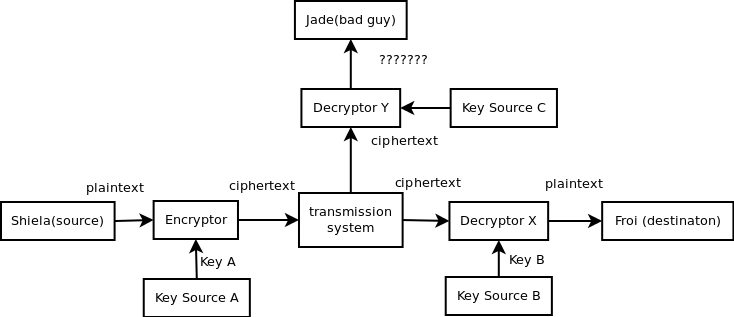
\includegraphics[scale=0.45]{flowchart1}
\end{figure}



\subsection{Merkle (1978)}

Secure communication, as described by Merkle\cite{merkle_secure_1978},
allows two parties to communicate in a private manner even though
a third party tries its best to learn what is being communicated.
We refer to the two parties as Froi and Shiela, and the third party
as Jade (Figure 5). Since the key channel is important, the following
describes the characteristics of the channel in relation to Jade.
\begin{enumerate}
\item All attempts by Jade to change the messages on the key channel are
detectable.
\item Jade will not be able to know the actual content of any message passing
on the key channel.
\end{enumerate}
The approach by Merkle relaxes the second condition: It is not necessary
for Jade not to know what is being sent in the key channel, he can
even know everything passing on it. The challenge then is how to securely
distribute the key satisfying the conditions above. If Froi and Shiela
have agreed upon a key, and the work needed by Jade to find the key
is much higher than the effort by Froi and Shiela needed to generate
the key , then it is a solution. The effort by Jade should be exponentially
higher compared to the effort by Froi or Shiela for a method to be
considered a solution. 

Merkle's method uses the concept of puzzles\cite{merkle_secure_1978}.
A puzzle is a cryptogram that is meant to be solved. Any encryption
function can be used to generate a puzzle. To allow the puzzle to
be solved, the key size (N) used in the encryption function is restricted.
The difficulty of solving a puzzle can be controlled by adjusting
the size of N. A very large size (in bits) of N will make it very
difficult to solve the puzzle. In addition, in order to be able to
solve the puzzle, some redundancy is needed. Redundancy is introduced
by encrypting, along with the original message, some constant known
to Froi, Shiela, and Jade. The absence of the constant when a puzzle
is decrypted would mean that a wrong key has been used. 

Let us consider the scenario when Shiela wishes to send a message
to Froi. First, they both agree on the value of N to use. Shiela then
generates N puzzles and transmits these N puzzles to Froi using the
key channel. Each puzzle generated will have a puzzle ID and puzzle
key. The puzzle ID uniquely identifies each puzzle. The puzzle key
on the other hand will be used in future communications that will
happen once this puzzle has been solved. 

When Froi receives the N puzzles, he selects a puzzle at random and
attempts to solve the puzzle, with the amount of effort required,
as defined by the size of the key space specified by Shiela. After
solving a puzzle, Froi sends the puzzle ID back to Shiela using the
key channel. The puzzle key, associated with the puzzle ID sent by
Froi, is then used for future communications, this time over the normal
channel. At this point Jade knows the puzzle ID, since it was sent
using the key channel, but not the puzzle key. If Jade wants to know
the key, then he must solve puzzles randomly and check the puzzle
ID if it matches the one sent by Froi back to Shiela. This will take
Jade a long time to solve. To put it formally, Jade will require $O(N^{2})$
effort to determine the key whereas Froi will only need, on the average,
$O(N)$. The function below generates the puzzles sent by Shiela to
Froi. The encryption function is arbitrary.

\begin{lstlisting}[language=C,numbers=left]
void generate_puzzle()
{
   bit_string id, key, c, random_key, puzzle, k1, k2;
   int i;

   k1 = rand(MAXINT);
   k2 = rand(MAXINT);
   c = rand(MAXINT);
   send(c);
   for (i=0; i<N; i++)
   {
      id = encryption_function(k1,i);
      key = encryption_function(k2, i);
      random_key = rand(c*N);
      puzzle = encryption_function(random_key,id,key,c);
      send(puzzle);
   }
}
\end{lstlisting}


The code below is executed on Froi's side.

\begin{lstlisting}[language=C,numbers=left]
void get_id()
{
   bit_string id, key, c, selected_puzzle_id, the_puzzle, current_puzzle,
              temp_constant;
   int i;
   
   selected_puzzle_id = rand(N);
   receive(c);
   for (i=0; i<N; i++)
   {
      receive(currrent_puzzle);
      if (i == selected_puzzle_id)
         the_puzzle = current_puzzle;
   }
   for (i=0;i<(c*N);i++)
   {
      id = get_id(finverse(i, the_puzzle));  
      key = get_key(finverse(i, the_puzzle));
      temp_constant = get_constant(finverse(i, the_puzzle));
      if (temp_constant == c)
         send(id);
   }
}
\end{lstlisting}


Once Shiela receives the the puzzle ID from Froi, then the following
code will be executed. key will be used for subsequent communications
between the two.

\begin{lstlisting}[language=C,numbers=left]
void continue_transmission()
{
   receive(ID);
   key = encryption_function(k2, ID);
}
\end{lstlisting}


The approach by Merkle requires an effort of $O(N^{2})$ from Jade
to get the key. However, in todays available computing resources,
this can be easily broken. The possibility of exponential methods
will be more attractive. Also the amount of information sent during
the initial setup of the communication is large because N puzzles,
consequently N keys, are sent initially.


\subsection{Diffie-Hellman (1976)}

The work by Diffie and Hellman\cite{diffie_new_1976} proposed a method
such that only one ``key'' needs to be exchanged and in addition
the time required from Jade to perform cryptanalysis is exponential.
In addition, it allows authentication because its use allows it to
be tied to a public file of user information. Shiela can authenticate
Froi and vice versa. 

Diffie and Hellman differentiate \textit{public key cryptosystems}
and \textit{public key distribution systems}. We let ${K}$ be the
finite key space from which keys $K$ can be obtained and ${M}$ be
the finite message space where messages $M$ are derived. A \textit{public
key cryptosystem} is a pair of families of algorithms ${E_{k}}$ and${D_{k}}$
which represent invertible transformations\cite{diffie_new_1976}.
\[
E_{k}:\{M\}\rightarrow\{M\}
\]


\[
D_{k}:\{M\}\rightarrow\{M\}
\]


such that 
\begin{enumerate}
\item for every key $K$, $E_{k}$ is the inverse of $D_{k}$,
\item for every $K$ and $M$, the algorithms $E_{k}$ and $D_{k}$ are
easy to compute,
\item for almost every $K$, each easily computed algorithm equivalent to
$D_{k}$ is computationally infeasible to derive from $E_{k}$,
\item for every $K$, it is feasible to compute inverse pairs $E_{k}$ and
$D_{k}$ from $K$.
\end{enumerate}
Property 3 allows $E_{k}$ to be made public without compromising
$D_{k}$. Key distribution in this system is simplified. Users generate
two keys, an enciphering key $E$ and a deciphering key $D$. $E$
can be made public but $D$ is kept privately by the user. Any entity
who would like to send messages to a user can use the publicly available
$E$ to encrypt messages but only the user can decrypt the message
using $D$. In their paper, Diffie and Hellman gave an example public
key cryptosystem by multiplying a binary n-vector message m with an
invertible binary n x n matrix E. However, this approach is not practical.

Merkle's\cite{merkle_secure_1978} work was classified by Diffie and
Hellman as \textit{public key distribution system} and highlighted
its limitations specifically its high transmission overhead again
because of sending N puzzles initially. The proposed system is similar
to the public key cryptosystem described above, but unlike Merkle's
technique, Diffie and Hellman approach allows the authentication of
users by making the public file read-only\cite{diffie_new_1976}. 

The technique proposed is dependent on the difficulty of computing
$logs\: mod\: q$ where q is a prime number representing the number
of elements of a finite field. Users generate independent random numbers
$X_{i}$ from the set of integers $\left\{ 1,2,...,q-1\right\} $.
The users keep these numbers but the computed value 
\[
Y_{i}=\alpha^{X_{i}}mod\: q
\]


is placed publicly together with the user information( such as name
and email). 

Consider for example Shiela and Froi would like to talk to each other
privately. They are going to use the key $K_{Shiela,Froi}$below after
they generate $X_{Shiela}$and $X_{Froi}$ and published $Y_{Shiela}$
and $Y_{Froi}$.

\[
K_{Shiela,Froi}=\alpha^{X_{Shiela}X_{Froi}}mod\: q
\]


Shiela will be able to obtain $K_{Shiela,Froi}$ by using the public
file $Y_{Froi}$ and then computing
\[
K_{Shiela,Froi}=Y_{Froi}^{X_{Shiela}}mod\: q
\]
 
\[
=(\alpha^{X_{Froi}})^{X_{Shiela}}mod\: q
\]


\[
=\alpha^{X_{Froi}X_{Shiela}}=\alpha^{X_{Shiela}X_{Froi}}mod\: q
\]


Froi will be able to obtain the key in the same manner. 
\[
K_{Sheila,Froi}=Y_{Shiela}^{X_{Froi}}mod\: q
\]
 

Jade might be able to compute$K_{Shiela,Froi}$ from $Y_{Shiela}$
and $Y_{Froi}$ by computing

\[
K_{Shiela,Froi}=Y_{Shiela}^{(\log_{\alpha}Y_{Froi})}mod\: q
\]


However, if Jade is to perform this computation, it will take him
a long time to do so. This system takes advantage of the fact that
$logs\: mod\: q$ are expensive to compute.


\subsection{Rivest-Shamir-Adleman (1978)}

The RSA algorithm by Rivest, Shamir, and Andleman was inspired by
the work of Diffie and Hellman. Despite the breakthrough in Diffie
and Hellman's work in public key cryptosystems, they did not present
any practical implementation that can be used in actual systems. The
creators of RSA took the work further by presenting a practical and
efficient implementation. Given an encryption procedure \textbf{E}
,a decryption procedure \textbf{D}, and a message \textbf{P}, a public
key cryptosystem has the following properties\cite{rivest_method_1978}:
\begin{enumerate}
\item Decrypting an encrypted \textbf{P} results to \textbf{P}. \textbf{D}(\textbf{E}(\textbf{P}))
= \textbf{P.}
\item \textbf{D} and \textbf{E} are easy to compute.
\item Publicly revealing \textbf{E} does not mean that it will be easy to
compute \textbf{D} from \textbf{E}. It should be difficult or inefficient
to compute \textbf{D} from \textbf{E}.
\item If \textbf{P} is decrypted and then encrypted, \textbf{P} is the result.
\textbf{E}(\textbf{D}(\textbf{P})) = \textbf{P}.
\end{enumerate}
The encryption and decryption functions rely on a key such that the
security of the functions or procedures rests on the security of the
key. If \textbf{E} satisfies properties 1-3 is referred to as ``trap-door
one way function''. If it also satisfies property 4 then it is referred
to as ``trap-door one-way permutation''. In public key cryptosystems
the usual ``setup'' time is simply the time it takes to make the
encryption function public.%
\footnote{In their paper, it is the encryption function that is made public.
Other researchers talk about keys being made public, not the functions.
Essentially, however, there is a one-to-one correspondence between
the encryption function and the key.%
} If Shiela wants to encrypt a message \textbf{P}, for Froi, with the
key \textbf{(e, n)}, she must first represent \textbf{P} as an integer
between \textbf{0} and \textbf{n-1}, where \textbf{e} and \textbf{n}
are positive integers. \textbf{P} is then encrypted to generate the
ciphertext \textbf{C} by raising \textbf{P} to the $e^{th}$ power
modulo \textbf{n}. The decryption process will raise the ciphertext
to another power \textbf{d} modulo \textbf{n}. The mathematical formulation
is shown below. 
\[
C\equiv E(P)\equiv P^{e}(mod\: n)
\]


\[
P\equiv D(C)\equiv C^{d}(mod\: n)
\]


The the length of the original message is not increased during the
encryption process. The pairs \textbf{(e,n)} and \textbf{(d,n)} are
the encryption keys and decryption keys respectively. The encryption
key is made public and the decryption key is private to the user.
In the above example, \textbf{(e,n)} is the public key of Froi, he
can decrypt the message using \textbf{(d,n)} which is in his possession.
The security of the approach is based on the security of the keys,
thus the keys must be selected well. \textbf{n} is computed as a product
of two large random primes \textbf{p} and \textbf{q}, \textbf{n =
p {*} q}. Although \textbf{n} will be made public, \textbf{p} and
\textbf{q} will not, which hides the way \textbf{d} can be derived
from \textbf{e}. \textbf{d} is a random integer such that $gcd(d,(p-1)*(q-1))=1$.
\textbf{e} is computed from \textbf{p}, \textbf{q}, and \textbf{d}
such that

\[
e*d\equiv1(mod(p-1)*(q-1))
\]


This requirement guarantees that properties 1 and 4 above are satisfied,
which means that \textbf{E} and \textbf{D} are inverse permutations.
Although Diffie and Hellman\cite{diffie_new_1976} also used exponentiation
and modulo in determining a common key to be used, their approach
is not based on a ``trap-door one-way permutation'' which means
that property 4 is satisfied.

The creators of RSA presented an efficient implementation of the of
their approach. Note that the basic operations in the encryption and
decryption process are exponentiation and division (to compute the
remainder). The technique is called ``exponentiation by repeated
squaring and multiplication.'' The technique presented will need
at most $2*\log_{2}(e)$ multiplications and $2*\log_{2}(e)$ divisions.
The encryption and decryption algorithms are shown below.
\begin{lstlisting}[language=C,numbers=left]
long E(long P,int e, int n)
{
   long C=1;
   int i;
   
   for (i=k;k==0;k--)
   {
      C = (C * C) % n;
      if (bit(i,e) == 1) /* bit(i,e) returns the ith bit of e*/
         C = (C * P) % n;
   }
   return C;  
}

long D(long C,int d, int n)
{
   long P=1;
   int i;
   
   for (i=k;k==0;k--)
   {
      P = (P * P) % n;
      if (bit(i,d) == 1) /* bit(i,d) returns the ith bit of d*/
         P = (P * C) % n;
   }
   return P;  
}
\end{lstlisting}


It can be seen that the RSA encryption and decryption algorithms are
straightforward to implement. The challenge however is in the selection
of the keys which is dependent of several parameters (e, d, n). In
their paper, the creators of RSA also presented several approaches
how to generate these parameters to guarantee the security.


\subsection{Elgamal(1985)\cite{elgamal_public_1985}}


\subsection{Elliptic Curve Cryptosystems(1987)\cite{koblitz_elliptic_1987}}

\bibliographystyle{plain}
\bibliography{asymmetric}

\end{document}
